[125~r\textsuperscript{o}]
residue avec la quelle il continue son mouuement, et avec la quelle 
%
%Zeile 10
%
il
\edtext{doit pousser}{\lemma{doit}\Bfootnote{\textit{(1)}\ chocquer \textit{(2)}\ pousser \textit{L}}}
le second moulinet \rule[-4mm]{0mm}{10mm}$\displaystyle E$ est $\displaystyle \frac{p}{p + \pi}v$. comme nous venons de dire. Appelons cette vistesse\protect\index{Sachverzeichnis}{vitesse}, $\displaystyle (v)$ et faisons
\rule[-4mm]{0mm}{10mm}\edtext{$\displaystyle \frac{p}{p + \pi}v \, \sqcap \, (v)$. Or}{\lemma{$\displaystyle \frac{p}{p + \pi}v \, \sqcap \, (v)$}\Bfootnote{\textit{(1)}\ par consequent \textit{(2)}\ . Or \textit{L}}}
la deminution de la vistesse par le second
\edtext{choc\protect\index{Sachverzeichnis}{choc} est}{\lemma{choc}\Bfootnote{\textit{(1)}\ sera \textit{(2)}\ est \textit{L}}}:
\rule[-4mm]{0mm}{10mm}$\displaystyle \frac{\pi}{p + \pi} (v)$ comme je viens de dire (voyez l'endroit marqu\'{e} de NB), donc au lieu de $\displaystyle (v)$ mettant sa valeur, nous aurons \rule[-4mm]{0mm}{10mm}$\displaystyle \frac{\pi p}{p^2 + 2p \pi + \pi ^2} v$. seconde diminution, et la vistesse residue avec la quelle le corps $\displaystyle A$ continue \`{a} passer estant \rule[-4mm]{0mm}{10mm}$\displaystyle \frac{p}{p + \pi} (v)$. expliquant $\displaystyle (v)$ par sa valeur \rule[-4mm]{0mm}{10mm}$\displaystyle \frac{p}{p + \pi} v$. nous aurons pour la vistesse 
rest\'{e}e
\edtext{$\displaystyle \frac{p^2}{p^2 + 2p \pi + \pi ^2} v$ ou la premiere vistesse 
%
%neue Seite
%
multipli\'{e}e par le quarr\'{e} de $\displaystyle \frac{p}{p + \pi}$. C'est \`{a} dire la vistesse rest\'{e}e apr\`{e}s le deuxieme choc sera \`{a} la premi\`{e}re en raison doubl\'{e}e de $\displaystyle p$ \`{a} $\displaystyle p + \pi$. Et le m\^{e}me calcul estant continu\'{e} on trouvera que la vistesse rest\'{e}e apr\`{e}s le troisieme choc sera $\displaystyle \frac{p^3}{p^3 + 3p^2 \pi + 3p \pi ^2 + \pi ^3 }, v$, c'est \`{a} dire la premiere $\displaystyle v$}{\lemma{$\displaystyle \frac{p^2}{p^2 + 2p \pi + \pi ^2} v$}\Bfootnote{\textit{(1)}\ ou le quarr\'{e} de $\displaystyle \frac{p}{p + \pi}$ \textit{(2)}\ . En continuant le m\^{e}me calcul on trouuera que la vistesse rest\'{e}e apr\`{e}s avoir pouss\'{e} le troisieme moulinet sera la premiere vi \textit{(3)}\ ou la premiere [...] apr\`{e}s \textbar\ le deuxieme choc \textit{erg.}\ \textbar\ sera [...] c'est \`{a} dire \textit{(a)}\ qu'elle sera \`{a} la premi\`{e}re comme \textit{(b)}\ la premiere $\displaystyle v$, \textit{L}}},
multipli\'{e}e par le cube de \rule[-4mm]{0mm}{10mm}$\displaystyle \frac{p}{p + \pi}$. ou qu'elle sera \`{a} la premiere vistesse 
%
%Zeile 5
%
$\displaystyle v$ en raison tripl\'{e}e de $\displaystyle p$ \`{a} $\displaystyle p + \pi$. Et ainsi de suite; le nombre des moulinets croissant arithmetiquement, la vistesse decroistra geometriquement. Donc conceuuant le
\edtext{nombre de ces moulinets}{\lemma{nombre}\Bfootnote{\textit{(1)}\ des mo \textit{(2)}\ de tels \textit{(3)}\ des obstacles tels que je con\c{c}ois ser \textit{(4)}\ de ces moulinets \textit{L}}},
infini et repet\'{e} en chaque endroit de l'espace, ou supposant les distances des moulinets infiniment petites et egales entre elles, c'est \`{a} dire supposant qu'un corps mû trouue une resistence\protect\index{Sachverzeichnis}{r\'{e}sistance} proportionelle \`{a} sa vistesse, les
\edtext{espaces croissant en progression 
%
%Zeile 10
%
arithmetique, les vistesses decroistront}{\lemma{espaces}\Bfootnote{\textit{(1)}\ estant comme les nombres, les vistesses rest \textit{(2)}\ croissant en progression \textit{(a)}\ Geometrique \textit{(b)}\ arithmetique, [...] decroistront \textit{L}}}
\edtext{ou leur [deminutions]\edtext{}{\Bfootnote{deminution \textit{\ L \"{a}ndert Hrsg.}}} croistront}{\lemma{}\Bfootnote{ou leur [...] croistront \textit{erg.} \textit{L}}}
en progression geometrique, \edtext{et par consequent les deminutions des vistesses estant}{\lemma{et}\Bfootnote{\textit{(1)}\ les espaces estant \textit{(2)}\ par consequent  \textit{(a)}\ les espaces estant \textit{(b)}\ les deminutions [...] estant \textit{L}}}
comme les nombres; les espaces parcourus\protect\index{Sachverzeichnis}{espace parcouru} seront comme leur logarithmes.\\
\pend
\pstart
\centering[\textit{Teil 3}]
\pend
\pstart
%
%Zeile 15
%
\noindent\edtext{Si}{\lemma{}\Bfootnote{\textit{(1)}\ Videamus \textit{(2)}\ Ex  \textit{(a)}\ iis \textit{(b)}\ his duobus satis explicatam habemus \textit{(3)}\ Si \textit{L}}}
corpus durum super alio duro et aspero incedere cogitemus, considerandum est primum eminentias illas esse elasticas, unde locum habet diminutio virium\protect\index{Sachverzeichnis}{vis} aequalis; esse etiam mole quadam praeditas, unde oritur diminutio celeritatum\protect\index{Sachverzeichnis}{celeritas} proportionalis; denique corpus dum premit nonnihil assurgere in ipsas eminentias, dum superat eas ac subjugat, et hac quidem ratione cogitandum est grave quasi per gradus quosdam
\edtext{ascendere, sed 
%
%Zeile 20
%
quoniam}{\lemma{ascendere,}\Bfootnote{\textit{(1)}\ (nam quod \textit{(2)}\ sed quoniam \textit{L}}}
rursus subsidit, eaque ipsa gravitate sua ad eminentias subjugandas contribuit, ascensus nihil perdet,
\edtext{alioquin perdidisset}{\lemma{alioquin}\Bfootnote{\textit{(1)}\ fuisset idem, ac si p \textit{(2)}\ perdidisset \textit{L}}}
tantundem celeritatis quantum perdit pendulum\protect\index{Sachverzeichnis}{pendulum}, descendendo per ima
\edtext{spatia,}{\lemma{}\Bfootnote{spatia, \textbar\ nimirum celeritates erunt quaesitae ultimae \textit{ gestr.}\ \textbar\ unde \textit{L}}}
unde alius plane oriretur calculus; sed eo non est opus.
\pend
\pstart
Quod attinet [ad]\edtext{}{\Bfootnote{in \textit{L \"{a}ndert Hrsg.}}}
motum in aere\protect\index{Sachverzeichnis}{aer} aut aqua\protect\index{Sachverzeichnis}{aqua}, cogitare licet eadem celeritate ferri non 
%
%Zeile 25
%
corpus, sed ipsum aerem
\edtext{[aut]}{\lemma{}\Bfootnote{aut \textit{erg.} \textit{Hrsg.}}}
ipsam \edtext{aquam, quiescente corpore, vel partem motus aquae seu aeri partem}{\lemma{aquam,}\Bfootnote{\textit{(1)}\ vel etiam partem \textit{(2)}\ quiescente [...] partem \textit{L}}}
corpori tribuere licet, quasi iret contra ventum aut contra flumen. Ictum 
%
%neue Seite
%
quem ventus flando \edtext{imprimit, aut aqua fluctu manifestum est esse majorem [125~v\textsuperscript{o}] cum major est celeritas.}{\lemma{imprimit,}\Bfootnote{\textit{(1)}\ necesse est \textit{(2)}\ aut aqua fluctu manifestum est  \textit{(a)}\ tanto esse majorem quanto \textit{(b)}\ esse [...] celeritas. \textit{L}}}
Itaque hinc sequitur necessario etiam magis obstare aquam\protect\index{Sachverzeichnis}{aqua} vel ventum\protect\index{Sachverzeichnis}{ventus} etsi quietum, motui corporis celeri quam tardo.
\pend
\pstart
Certum est liquida alia aliis majorem infligere ictum\protect\index{Sachverzeichnis}{ictus}, quod scilicet alia aliis densiora
%
%Zeile 5
%
 \edtext{sunt. Causa utique}{\lemma{sunt.}\Bfootnote{\textit{(1)}\ Ita \textit{(2)}\ Duo \textit{(3)}\ Causa utique \textit{L}}}
quae facit ut liquidum motui corporis resistat, vel quod idem est, ut liquidum ictum solido infligat, nulla est alia quam quod mobile in liquido progredi non potest, quin motum quendam peculiarem in partibus liquidi \edtext{producat. Cum}{\lemma{producat.}\Bfootnote{\textit{(1)}\ Nam et \textit{(2)}\ Cum \textit{L}}}
jactum aquae aut flatum aeris\protect\index{Sachverzeichnis}{aer} sustinet, experimenta sumenda sunt, an vis\protect\index{Sachverzeichnis}{vis} exerceatur non a longitudine, sed tantum a largitate seu crassitie, et celeritate ictus. Quod arbitror, nempe jactum 
%
%Zeile 10
%
longum ejusdem crassitiei et celeritatis non plus facere quam brevem. Hinc sequitur non impingentis aquae magnitudinem, sed soliditatem sive densitatem \edtext{specificam celeritati}{\lemma{specificam}\Bfootnote{\textit{(1)}\ gravitati \textit{(2)}\ celeritati \textit{L}}}
junctam esse causam ictus magni. Id est materiae liquidae\protect\index{Sachverzeichnis}{materia liquida} jactae detorsionem a linea jactus per quietem corporis obstantis esse causam motus corporis. Vim \edtext{ergo ictus per jactum}{\lemma{ergo}\Bfootnote{\textit{(1)}\ jactus \textit{(2)}\ ictus per jactum \textit{L}}}
ex eo aestimabimus quod fieret corpore obstante posito immobili. Fingamus autem 
%
%Zeile 15
%
aquam quae ictum infligere dicenda \edtext{est sequenti alia aqua non}{\lemma{est}\Bfootnote{\textit{(1)}\ ictu sequenti non \textit{(2)}\ sequenti alia aqua non \textit{L}}}
urgeri. Non potest ictus intelligi factus, nisi a globulis\protect\index{Sachverzeichnis}{globulus} illis paucis impingentibus quorum motus
\edtext{detorquetur}{\lemma{}\Bfootnote{detorquetur \textit{erg.} \textit{L}}}
in quantum superficiei corporis objecti perpendicularis est, aut ab illis quae ipsis immediate sunt continua.
Equidem credo tuto de liquidis explicari quae de pulverea nube dici possunt aut de fumo aliaque corpusculorum\protect\index{Sachverzeichnis}{corpusculum} confluge.
\pend
\pstart
%
%Zeile 20
%
    Nec tantum considerandum est, quod aliquot \edtext{globuli retineantur}{\lemma{globuli}\Bfootnote{\textit{(1)}\ impingunt \textit{(2)}\ retineantur \textit{L}}},
sed et quod inter \edtext{hos aliosque}{\lemma{hos}\Bfootnote{\textit{(1)}\ aliquosque \textit{(2)}\ aliosque \textit{L}}}
aliqua conjunctio sive glutinositas, ut alter sine altero non facile moveatur.
\begin{wrapfigure}[9]{l}{0.36\textwidth}    
    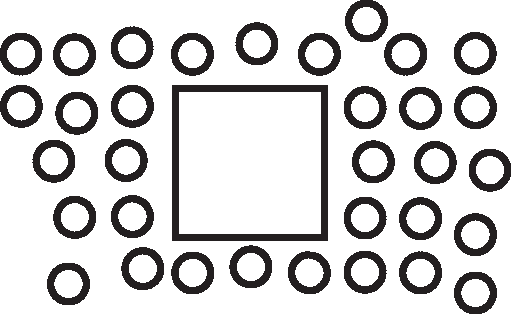
\includegraphics[trim = 0mm -5mm -8mm 0mm, clip, width=0.36\textwidth]{images/lh0351402_125-d1.pdf}
    \centering [\textit{Fig. 4}]% \caption{Bildbeschreibung}
    \end{wrapfigure}
Sed quanta aut qualiacunque haec sint semper eodem modo intelligi possunt. Itaque cognita liquoris specie quaeritur tum de quantitate ictus, tum de numero 
%
%Zeile 25
%
supervenientium ictuum. Jam quanto celerior est liquidi motus eo plures eodem tempore superveniunt ictus, sunt ergo \edtext{ictus tam magnitudine quam numero ut celeritates adeoque in duplicata celeritatum}{\lemma{ictus}\Bfootnote{\textit{(1)}\ in duplicata celeritatum. Primum ergo movetur corpus \textit{(2)}\ tam magnitudine [...] celeritatum. \textit{L}}}.
Sermo autem est non de celeritate absoluta sed respectiva seu accessu, itaque corpore ipso motum recipiente a mobili 
%
%neue Seite
%
et simul eunte minuitur celeritas, donec postremo ictus fiat nullus cum nulla superest celeritas respectiva, seu percussio, seu cum simul moventur. Nimirum cum initio corpus in liquore medio positum unum acceperit ictum, movetur sane, sed tarde, secundo ictu rursus, celerius; tertio majorem iterum \edtext{acquirit a}{\lemma{acquirit}\Bfootnote{\textit{(1)}\ ab \textit{(2)}\ a \textit{L}}}
percussione celeritatem, donec \edtext{ad}{\lemma{}\Bfootnote{ad \textit{erg.} \textit{L}}}
%
%Zeile 5
%
eandem perveniat celeritatem cum liquido circumfuso, id est ad quietem quam servat, quoniam ex eo tempore cessat percussio\protect\index{Sachverzeichnis}{percussio}. \edtext{Itaque si}{\lemma{Itaque}\Bfootnote{\textit{(1)}\ quemadmodum \textit{(2)}\ si \textit{L}}}
quolibet temporis momento novum fieri ictum imaginemur, opus est etiam partem materiae primum impingentem esse infinite parvam, alioqui tempore minore quam quod intelligi possit motum aequalem liquido circumfuso mobile nancisceretur. At vero materiam impingentem esse infinite parvam 
%
%Zeile 10
%
impossibile est, neque enim \edtext{puncta sola}{\lemma{puncta}\Bfootnote{\textit{(1)}\ solida \textit{(2)}\ sola \textit{L}}}
volitare possunt, itaque etiam necesse \edtext{est ictus}{\lemma{est}\Bfootnote{\textit{(1)}\ ictum \textit{(2)}\ ictus \textit{L}}}
fieri per \edtext{intervalla. Haec si liquidum ex pulveriis ramentis compositum cogitemus}{\lemma{intervalla.}\Bfootnote{\textit{(1)}\ At si fingeremus  \textit{(a)}\ spatiu \textit{(b)}\ liquid \textit{(2)}\ Haec [...] cogitemus \textit{L}}},
sed si continuum esse fingamus cogitandum est ictum non alia de causa infligi, quam quod ab interposito corpore turbatur liquidi motus partesque divertuntur. Erit quoque liquidum perfectum, si fingamus divisum in particulas usque infinite parvas ubi sane intelligi 
%
%Zeile 15
%
potest quolibet temporis momento novum sequi ictum. Glutinositas aliqua sive connexio partium in liquido si ponatur, hoc tantum efficiet, ut eo plures sint partes impingentes ob connexionem, et magis etiam quo firmior connexio. Partem enim ictus in se recipiet id, quod est causa connexionis.
\pend
\pstart
Ut ad calculum motus nostri veniamus, sit mobilis moles\protect\index{Sachverzeichnis}{moles} expressa, $\displaystyle m$. portio 
%
%Zeile 20
%
liquidi impingens $\displaystyle l$. celeritas liquidi $\displaystyle v$. ejus momentum\protect\index{Sachverzeichnis}{momentum} $\displaystyle lv$. celeritas post ictum \rule[-4mm]{0mm}{10mm}$\displaystyle \frac{l}{l + m} v$. distantia primi impingentis et corporis $\displaystyle \delta$, tempus quo ea distantia absolvitur, $\displaystyle \theta$. Si mobile nullum accepisset ictum \edtext{tunc}{\lemma{}\Bfootnote{tunc \textit{erg.} \textit{L}}} tempore $\displaystyle \theta$, novus secutus fuisset ictus aequalis priori. Nunc vero quoniam etiam ipsum mobile quod excipere debet, antecedit, hinc perinde est ac si id quod impingere debet tantodem ferretur tardius (nam quantum ad 
%
%Zeile 25
%
percussionem perinde est cui des motum) celeritas ergo percussionis secundae portionis liquidi erit \rule[-4mm]{0mm}{10mm}$\displaystyle v - \frac{l}{l + m} v \ \sqcap \ \frac{vl + mv - vl}{l + m}$ sive $\displaystyle \frac{m}{l + m} v$. qua scilicet celeritate idem absolvit spatium\protect\index{Sachverzeichnis}{spatium} $\displaystyle \delta$. Fingimus enim ictu accepto non tam mobile promoveri, quam sequens impingens \edtext{retardari. Itaque momentum 2\textsuperscript{di} $\displaystyle l$ erit}{\lemma{retardari}\Bfootnote{\textit{(1)}\ et erit celeritas accepta post ictum \textit{(2)}\ . Itaque [...] erit \textit{L}}}
\rule[-4mm]{0mm}{10mm}$\displaystyle \frac{ml}{l + m} v$ et cum nunc non tantum se, sed et $\displaystyle m$, et primum $\displaystyle l$ moveat, hinc ejus momentum \edtext{erit dividendum per}{\lemma{erit}\Bfootnote{\textit{(1)}\ multiplicandum per \textit{(2)}\ dividendum per \textit{L}}}
materiam nempe 
%
%neue Seite
%
$\displaystyle m + 2l$. et fiet celeritas residua: \rule[-4mm]{0mm}{10mm}$\displaystyle \frac{ml}{\begin{array}{lll} m^2 & + \, 2ml & + \, l^2\\ & +\, 1 & +\, l^2 \end{array}} \begin{array}{r}\!\!\!v \end{array}$quae rursus ablata ab $\displaystyle v$ tertii liquidi relinquet \rule[-4mm]{0mm}{10mm}\edtext{$\displaystyle \frac{m^2 + 2ml + 2l^2}{m^2 + 3ml + 2l^2} v$. quod}{\lemma{$\displaystyle \frac{m^2 + 2ml + 2l^2}{m^2 + 3ml + 2l^2} v$}\Bfootnote{\textit{(1)}\ momentum \textit{(2)}\ . quod \textit{L}}}
iterum multiplicetur per $\displaystyle l$. dividatur per $\displaystyle m + 3l$
et \rule[-4mm]{0mm}{10mm} \edtext{fiet: $\displaystyle \frac{m^2 + 2ml + 2l^2}{\protect \begin{array}{llll} m^3 & + \, 3m^2 l & + \, 2l^2 m & + \, 6l^3\\ & + \, 3 \dots & + \, [9] \dots \protect \end{array}} \protect \begin{array}{r}\!\!\!lv.\protect \end{array}$}{\lemma{fiet:}\Bfootnote{\textit{(1)}\ $\displaystyle \frac{m + l^2}{m^2 + 3ml + 2l^2}lv + \frac{l^2}{m^2 + 3}lv$ \textit{(2)}\ $\displaystyle \frac{m^2 + 2ml + 2l^2}{\protect \begin{array}{llll} m^3 & + \, 3m^2 l & + \, 2l^2 m & + \, 6l^3\\ & + \, 3 \dots & + \, [9] \dots \protect \end{array}} \protect \begin{array}{r} lv \protect \end{array}$
\textit{L}}}\edtext{}{\Bfootnote{$\displaystyle + \, 6 \, \dots$ \textit{\ L \"{a}ndert Hrsg.}}}Et ita continuandus semper esset motus si corpusculis $\displaystyle l$ ipsum $\displaystyle m$ velut crescere fingamus pulvisculis quodammodo collectis, sed 
%
%Zeile5
%
reapse sciendum est pulvisculos illos $\displaystyle l$ ob liquiditatem seu \edtext{extremam liquiditatem, a supervenientium ictu}{\lemma{extremam liquiditatem,}\Bfootnote{\textit{(1)}\ ob m \textit{(2)}\ a supervenientium ictu \textit{L}}}
elidi, quamquam aliqui semper maneant interjecti et velut semper tantundem ob supervenientes novos.
Itaque perinde est ac si initio corpus $\displaystyle m$ ponamus paulo majus calculo caetera invariato, \edtext{itaque celeritas residua}{\lemma{itaque}\Bfootnote{\textit{(1)}\ moveatur \textit{(2)}\ celeritas residua \textit{L}}}
post ictum secundi liquidi erit: \rule[-4mm]{0mm}{10mm}$\displaystyle \frac{ml}{m + l, \, \boxed{\phantom{\scriptstyle{2}}}} v$. adimendo ab $\displaystyle v$ \edtext{restabit momentum}{\lemma{restabit}\Bfootnote{\textit{(1)}\ celeritas \textit{(2)}\ momentum \textit{ L}}}
tertii liquidi%\pend